\documentclass[10pt]{article}
\usepackage[table]{xcolor}
\usepackage{tikz}
\usetikzlibrary{arrows,automata}
\usepackage[latin1]{inputenc}
\usepackage{amsmath,amssymb}
\usepackage{color}

\begin{document}

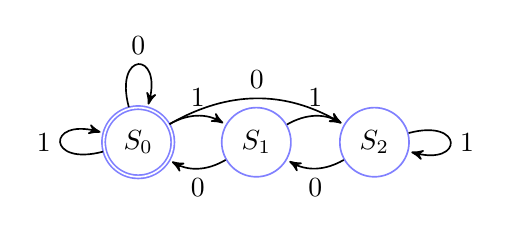
\begin{tikzpicture}[->,>=stealth',shorten >=1pt,auto,node distance=1.5cm,
                    semithick]
  \tikzstyle{every state}=[fill=white,draw=blue!50,text=black]

  \node[state,accepting]  (A)                    {$S_0$};
  \node[state]         (B) [right of=A]       {$S_1$};
  \node[state]         (C) [right of=B]       {$S_2$};

  \path (A) edge [bend left]              node {1} (B)
		edge [loop above]           node {0} (A)
        edge [loop left]            node {1} (A)
        edge [bend left]               node {0} (C)
        (B) edge [bend left]          node {1} (C)
        edge [bend left]          node {0} (A)
        (C) edge [bend left]          node {0} (B)
		edge [loop right]           node {1} (C);
\end{tikzpicture}

\end{document}